% \vspace{-2mm}
\section{Introduction}
\label{sec:intro}
% \vspace{-3mm}
\begin{figure}[t]
    \centering
    % \vspace{-3mm}
    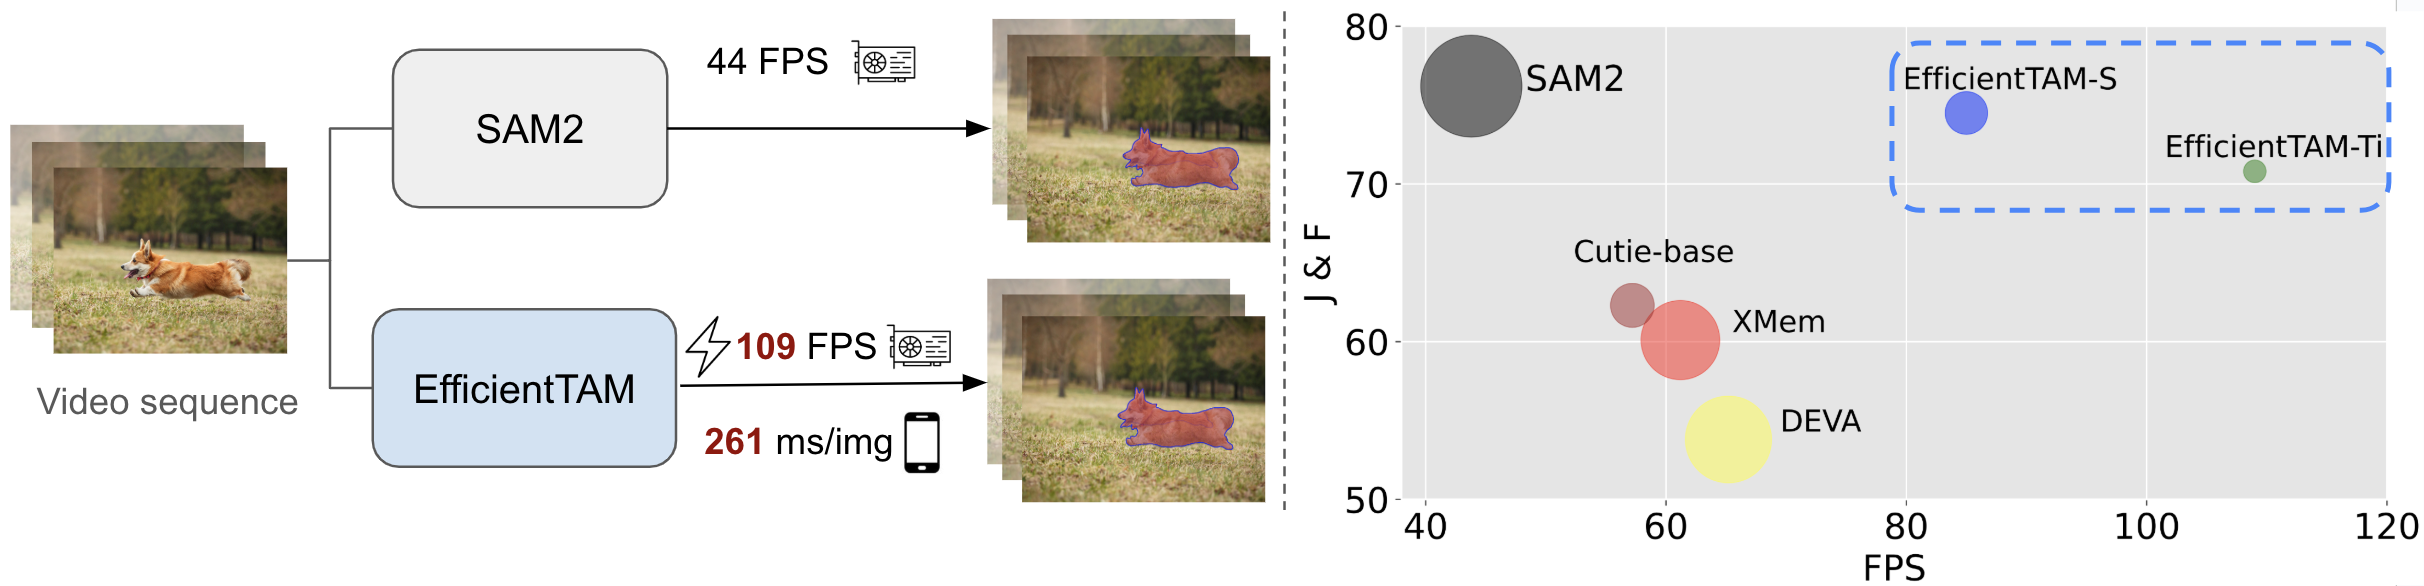
\includegraphics[width=\linewidth]{figures/intro.png}
    \caption{Comparative analysis. (Left) Speed comparison between EfficientTAM and SAM 2 on a single NVIDIA A100 GPU. While SAM 2 is challenging for on-device deployment, our EfficientTAM can run 261 ms per frame on iPhone 15 Pro Max. (Right) 
    FPS/Parameter/Performance comparison of EfficientTAM, SAM 2, and other efficient models for zero-shot video object segmentation on SA-V test. We benchmark FPS (frames per second) of all models with 1024 × 1024 input resolution on a single NVIDIA A100.}
    \label{fig:throughput}
% \vspace{-3mm}
\end{figure}

Segment Anything Model 2 (SAM 2)~\citep{ravi2024sam} is a foundational model for unified image and video object segmentation, achieving state-of-the-art performance in various segmentation tasks such as zero-shot image segmentation~\citep{kirillov2023segment,chen2023semantic,deng2023segment,chen2023sam}, semi-supervised video object segmentation~\citep{pont20172017,xu2018youtube,oh2019video,bhat2020learning,robinson2020learning,li2022recurrent,yang2022decoupling,cheng2022xmem,zhang2023joint,wang2023look,wu2023scalable,cheng2024putting,yang2024scalable}, interactive video segmentation~\citep{caelles20182018,heo2020interactive,cheng2021modular,homayounfar2021videoclick,yang2023track,cheng2023segment,rajivc2023segment,cheng2024putting,delatolas2024learning}, and other real-world applications~\citep{zhang2024evf,xiong2024sam2,shen2024performance,zhang2024sam2,ding2024sam2long,qiu2024ded,tang2024segment,zhou2024sam2}. SAM 2 uses a multistage image encoder  to extract hierarchical frame features and introduces a memory module to cross-attend to both current frame features and stored memories from observed frames for consistent object segmentation across frames and interactive tracking in videos. 
%This makes SAM 2 a vision foundation model and enables its applications beyond vision. 

Despite these advantages, SAM 2 is not efficient for mobile deployment, particularly because the large image encoder (e.g., HieraB+) and memory module are expensive. The default image encoder of SAM 2, HieraB+~\citep{ryali2023hiera}, is parameter inefficient, e.g., $\sim$80M parameters. While SAM 2 provides a tiny version, it has a running time of 43.8 FPS comparable to 47.2 FPS of the default SAM 2 model, due to the hierarchical image encoder. Additionally, that the memory tokens (e.g., a concatenation of spatial memory tokens and object pointer tokens) are long, e.g., $\sim$30K, which hurts the efficiency of the memory module with cross-attention. 
%Consequently, SAM 2 has high memory and computational costs when performing video object segmentation and track anything tasks, which makes it challenging for on-device applications. 

In this paper, we revisit plain, nonhierarchical image encoder for video object segmentation and tracking anything. We propose using a lightweight vanilla ViT image encoder (e.g., ViT-Tiny/-Small\citep{touvron2021training}) as EfficientSAMs\citep{xiong2024efficientsam} did to reduce the complexity of SAM 2 while maintaining decent performance. Further, we propose an efficient cross-attention method for accelerating the memory module. This is achieved by leveraging the underlying structure of memory spatial tokens. We observed that the memory spatial tokens have strong locality and a coarser representation of memory spatial tokens can be a good proxy for performing cross-attention. We show that this yields a good alternative to the original memory module. 

To evaluate our method, we conduct extensive experiments across video and image segmentation benchmarks, including MOSE, DAVIS, LVOS, and SA-V for video segmentation, and SA-23 for image segmentation. Our EfficientTAM outperforms strong semi-supervised video object segmentation methods such as Cutie-base, XMem, and DEVA while being more efficient. Compared with SAM 2, our EfficientTAM is comparable, e.g., 74.5\% vs 74.7\% on SA-V test dataset, with $\sim$ 2x reduced FPS. On image segmentation benchmark, SA-23, our EfficientTAM achieves 60.7\% accuracy for zero-shot image segmentation compared to 59.1\% accuracy for SAM and and 61.9\% for SAM 2. We also benchmarked our EfficientTAM model on iPhone 15 Pro Max, which can run $\sim$ 10 frames per second with reasonable video segmentation performance.
% compared to x frames per second for SAM and SAM 2. 

Our main contributions can be summarized as follows:
\begin{itemize}[noitemsep,topsep=0pt,leftmargin=0.5cm]
    \item 
    We revisit using plain, non-hierarchical image encoder, ViT-Tiny/-Small for video object segmentation and show that vanilla ViT can achieve competing performance comparing to SAM 2 with hierarchical image encoder. 
    
    
    \item We propose an efficient memory cross-attention by exploiting the underlying memory spatial token structure and demonstrate the favorable performance. 
    
    
    \item We deliver EfficientTAMs, lightweight video object segmentation and track anything models with state-of-the-art quality-efficiency tradeoffs (\cref{fig:throughput}), which is complementary to SAM 2 for practical deployment. 
    % Code and models will be released to benefit a wide range of efficient TAM applications. 
    
\end{itemize}

